\documentclass{report}
\usepackage[french]{babel}
\usepackage{graphicx}
\usepackage[utf8]{inputenc}
\usepackage{float}
\usepackage{array}
\usepackage{tabularx}
\usepackage[T1]{fontenc}
\usepackage{xcolor}
\usepackage{multirow}


\def\code#1{\texttt{#1}} % pour écrire du code (police monospace)
\def\comment#1{\color{gray} #1 \color{black}}

\begin{document}
\renewcommand{\labelitemi}{$\bullet$}
\renewcommand{\labelitemii}{$\circ$}
\thispagestyle{empty}

\begin{center}
	\vspace*{1cm}
	\huge  \bf Rapport du TP2: Paralèlliser un algorithme de filtrage numérique basé
	sur des opérations de convolution\\
	\vspace{1cm}

	\LARGE Equipe numéro 2\\
	\vspace{1.5cm}
	\normalsize
	\textit{Houssem Sebouai}\\
	111 134 915\\
	houssem.sebouai.1@ulaval.ca\\

  \vspace{1cm}
	\normalsize
	\textit{Thierry St-Gelais}\\
111 169 338\\
thierry.st-gelais.1@ulaval.ca\\

	\vspace{2cm}
	Dans le cadre des travaux pratiques du cours\\
	\LARGE GLO-7014\\
	\large Programmation parallèle et distribuée\\
	Professeur: Marc Parizeau

	\vfill
	
\includegraphics[width=5cm]{Images/logo.jpg}
	\\
	Hiver 2017
\end{center}

\newpage

\tableofcontents
\listoffigures
\listoftables
\newpage
\chapter{Introduction}
Dans ce deuxième travail pratique, nous avons été amener à paralléliser un algorithme
de filtrage numérique basé sur des opérations de convolution. Nous avons utilisée OpenMP
pour effectuer cette tache.
\chapter{Réalisation du travail pratique}
\section{Description générale de l'algorithme}
L'algorithme de filtrage se base principalement sur des opérations de convolution entre matrices
 sur les pixels d'une image en entrée pour produire une image en output.\\
Cette opération de convolution est applique selon un noyau (un noyau flou ou un noyau identité).
\section{Approche adoptée pour la parallélisation }
Dans notre approche du problème, nous avons choisi de paralléliser les deux premières
boucles imbriquées, en utilisant la clause "collapse".\\
Nous avons aussi choisi la stratégie statique pour la distribution des blocs de traitement
que chaque "thread" devera exécuter. Nous avons aussi défini aussi les variables {\it lR, lG, lB} 
comme étant des variables privées à chacun thread pour le calcul de la convolution.
\section{Expérimentations et résultats}
\subsection{Protocole d'expérimentation}
Pour nos expérimentations, nous avons choisi:
\begin{itemize}
	\item Une image plus significative en matière de nombre de pixels;
	\item Répéter le filtrage plusieurs fois d'affilée.
\end{itemize}
Ces choix nous permettent des mesures de performance en secondes plus
tot que des mesures en mellisecondes.

\subsection{Résultats}

\bigskip Suite à plusieurs expérimentations, nous en sommes arrivés aux résultats présentés sur les graphiques suivants:

\begin{center}
	\begin{figure}[H]
		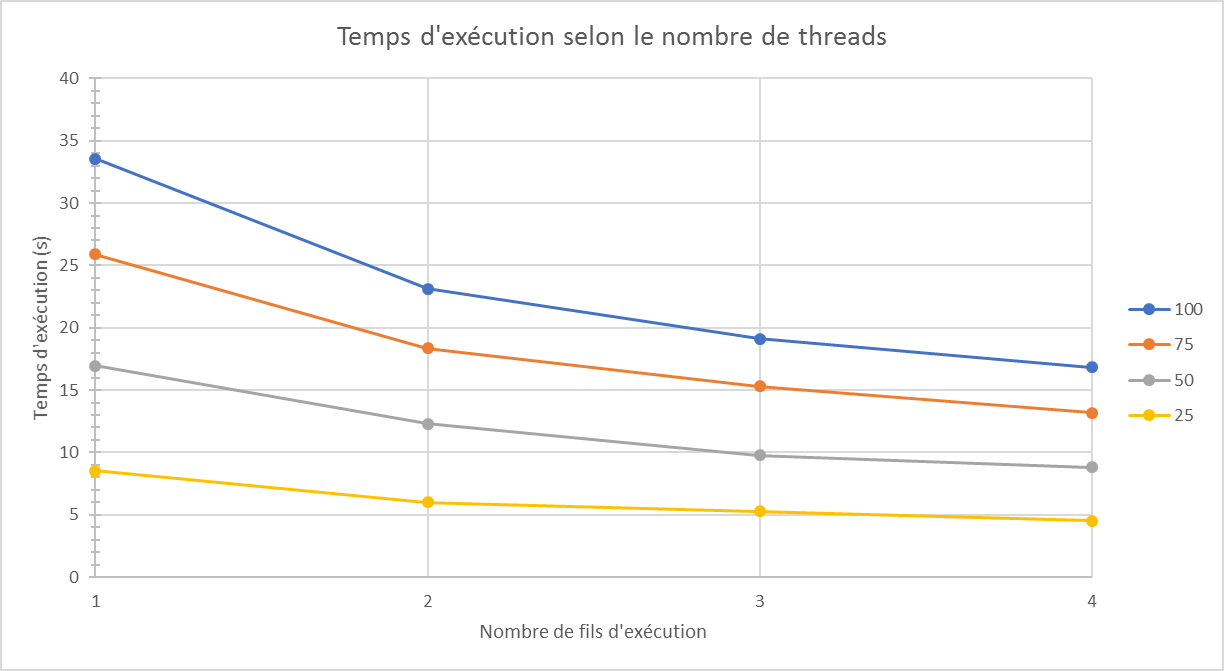
\includegraphics[scale=0.55]{Images/graph_temps.png}
		\caption{Temps d'exécution selon le nombre de fils pour un nombre donné d'exécutions}
	\end{figure}

	\begin{figure}[H]
		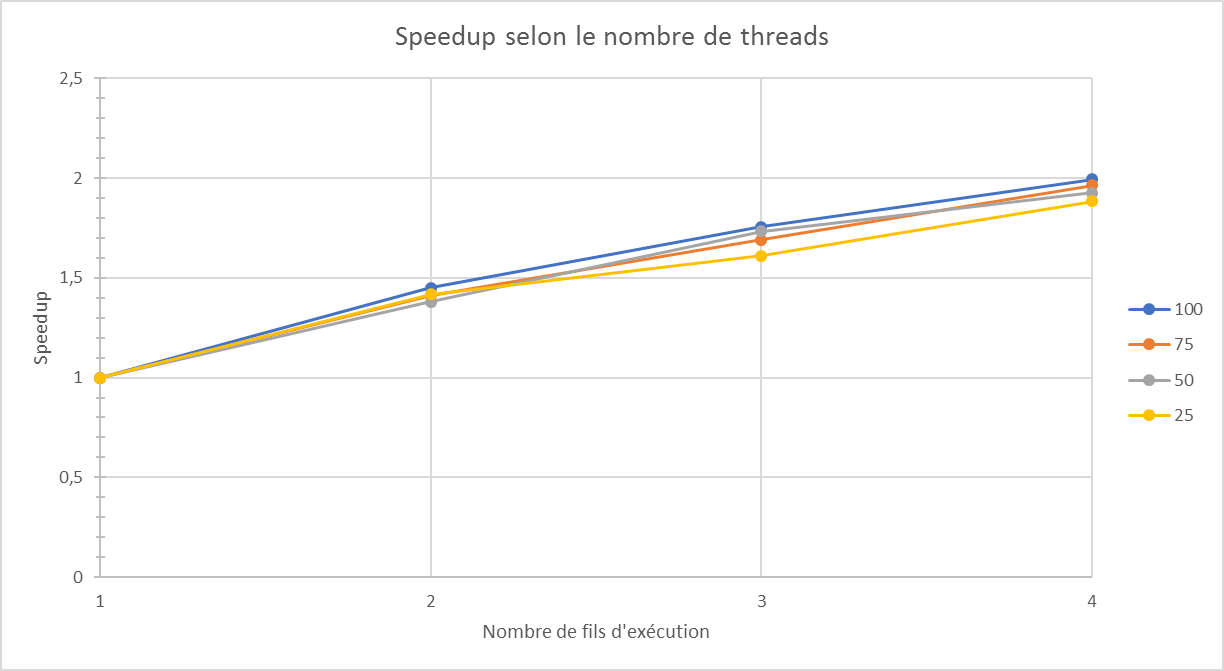
\includegraphics[scale=0.55]{Images/graph_speedup.png}
		\caption{Speedup selon le nombre de fils pour un nombre donné d'exécutions}
	\end{figure}

	\begin{figure}[H]
		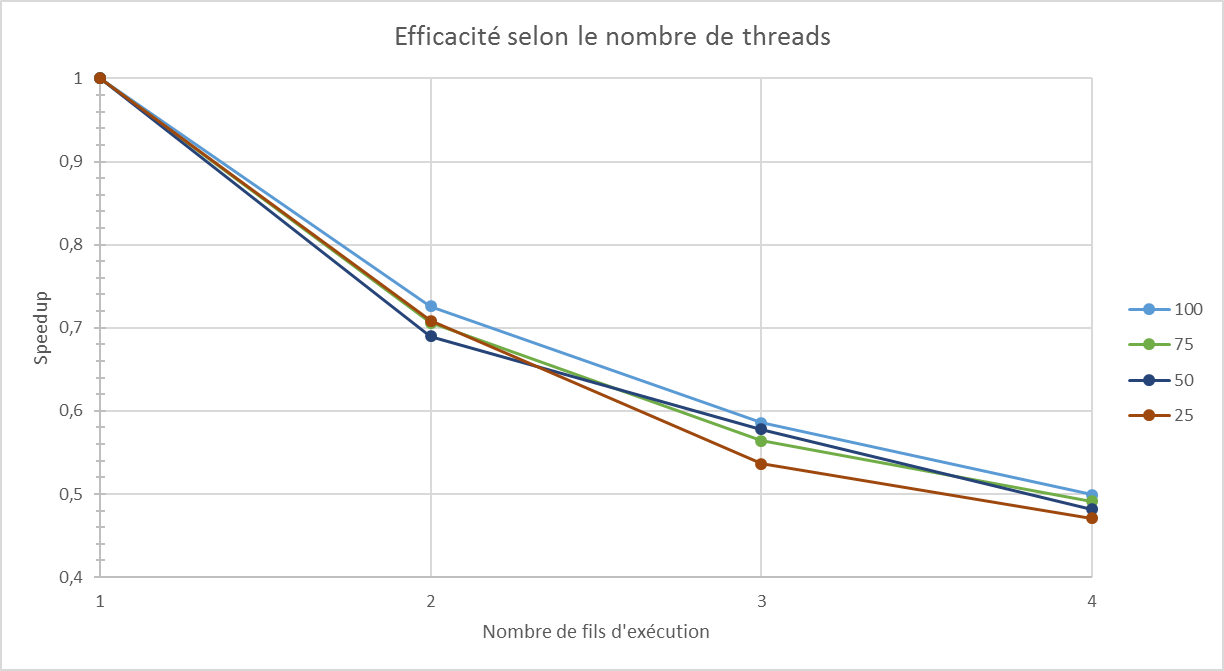
\includegraphics[scale=0.55]{Images/graph_eff.png}
		\caption{Efficacité selon le nombre de fils pour un nombre donné d'exécutions}
	\end{figure}
\end{center}

\subsection{Interprétation}

Ce que les trois graphiques précédent nous apprennent, c'est que notre algorithme voit son efficacité baisser assez rapidement selon le nombre de threads associées au processus. En effet, les courbes semblment montrer un plafonnement assez rapide de la diminution du temps d'exécution, ce qui ammène par le fait même un plafonnement du speedup et un plancher de l'efficacité de l'algorithme. Les tests effectués montrent un speedup maximal d'environ $2.5$ pour $X$ threads, bien que ceci ne soit pas démontré dans les graphiques. On obtient à ce moment une efficacité d'environ $0.313$. 

\bigskip Ces chiffres, quant à eux, nous portent à croire que l'algorithme est peu parallélisable, ce qui expliquerait le speedup et l'efficacité faibles.

\chapter{Conclusion}
Dans ce travail, nous avons essayé d'explorer ce qu'OpenMP offrait comme possibilités pour
paralléliser principalement des boucles, afin d'accélérer les calculs applique au filtrage
numérique d'image.
\end{document}
